\newpage
	\section{S} \label{sec:S}
	
		\subsection{SCALABILITÀ} \index{Scalabilità} \label{scalabitlita}
		Garantisce prestazioni.
		
		\subsection{SEMAT} \index{SEMAT} \label{semat}
			\textit{Software Engineering Method and Theory} fornisce teorie, principi provati e \underline{\hyperref[best]{best practices}} per l'ingegneria del software.
		
		\subsection{SISTEMA DI QUALITÁ} \index{Sistema di qualità} \label{sistemadiqualita}
		Riferimenti OGGETTIVI che ci dicono come stiamo lavorando.
		
		\subsection{SLACK} \index{Slack} \label{slack}
		Letteralmente:"lasco"; margine che posso consumare.
		
		\subsection{SOFTWARE DETERMINISTICO} \index{Software deterministico} \label{softwaredeterministico} 
		In ogni stato in cui mi trovo, so che posso avere solo "un'uscita". Devo sempre sapere lo stato in cui sono, quindi quello che mi precede e quello seguente.
		
		
		\subsection{SOFTWARE ENGINEERING} \index{Software Engineering} \label{swe}
	     L'\underline{\hyperref[engineering]{Ingegneria}} del Software è una disciplina volta a realizzare  \underline{\hyperref[prodotto]{prodotti software}} talmente impegnativi da richiedere lo svolgimento di attività collaborative. Agisce garantendo \underline{\hyperref[efficacia]{efficacia}} ed \underline{\hyperref[efficienza]{efficienza}} durante tutto il \underline{\hyperref[ciclo]{ciclo di vita}} del prodotto. È importante sottolineare che SWE non ha a che vedere solo con l'informatica, ma anche con alcune aree della matematica discreta, ricerca, statistica, psicologia ed economia. SWE inoltre adotta un determinato \underline{\hyperref[approccio]{approccio}}.
		
		\subsection{SOFTWARE SYSTEM} \index{Sistema software} \label{sistemasoftware} 
		Soluzione realizzabile (concretizza \underline{\hyperref[requirements]{requirements}}).
		
		\subsection{SOLUTION} \index{Solution} \label{solution}
		Secondo elemento di un progetto. Comprende \underline{\hyperref[requirements]{requirements}} e \underline{\hyperref[sistemasoftware]{software system}}.
		
		\subsection{STAKEHOLDER} \index{Stakeholder} \label{stakeholder} 
		(=portatori di interesse) Persone influenti: dicono se una certa \underline{\hyperref[opportunity]{opportunità}} è buona. Possono essere chi usa il prodotto (clienti), chi compra il prodotto (committente), chi sostiene i costi di realizzazione (fornitore), chi verifica l'attuazione di processi (eventuali regolatori).
		
		\subsection{STANDARD DI PROCESSO} \index{Standard di processo} \label{standard} 
		Nascono per iniziativa del committente al fine di facilitare controllo, collaudo e accettazione. Esistono standard come \textit{modello di azione} (che definiscono procedure o processi) e come \textit{modello di valutazione} (che sono modelli più generali e identificano la \underline{\hyperref[bes]{best practice}}).
		
			\subsubsection{ISO 12207}	\label{12207}
			È un modello di azione ed il modello più noto. Contiene tutti i processi significativi ad alto livello: identifica i processi di ciclo di vita del \underline{\hyperref[prodotto]{software}}, ha struttura modulare, specifica le responsabilità sui processi e i prodotti dei processi.
			
			\begin{figure}[H]
				\centering
				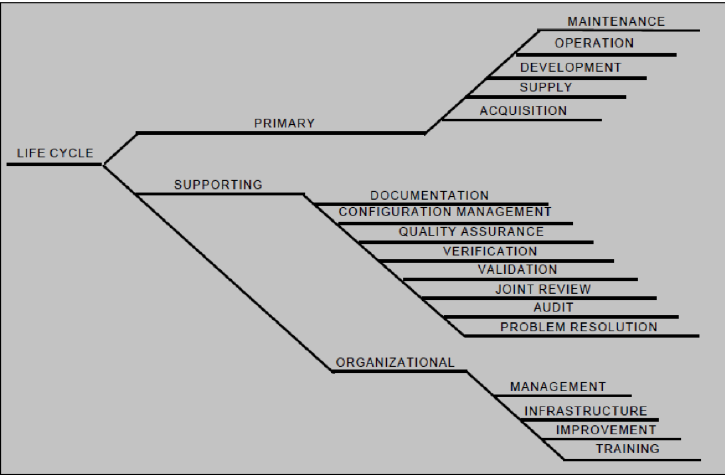
\includegraphics[width=0.78\textwidth]{img/iso}		
				\caption{Primary, supporting and organisational life-cycle processes.}
			\end{figure} 
			
			Almeno un \textit{processo primario} deve sempre esistere:
				\begin{itemize}
					\item \textbf{Acquisizione}: gestione dei sotto-fornitori;
					\item \textbf{Fornitura}: gestione dei rapporti con il cliente;
					\item \textbf{Sviluppo}: non è sempre detto che abbia rapporti con il cliente;
					\item \textbf{Gestione operativa/utilizzo}: installazione ed erogazione dei prodotti;
					\item \textbf{\underline{\hyperref[manutenzione]{Manutenzione}}};
				\end{itemize}
			
			\textit{Processi di supporto}:
				\begin{itemize}
					\item \textbf{Documentazione};
					\item \textbf{Accertamento della \underline{\hyperref[qualita]{qualità}}};
					\item \textbf{Gestione delle \underline{\hyperref[versione]{versioni}} e delle \underline{\hyperref[configurazione]{configurazioni}}};
					\item \textbf{\underline{\hyperref[verificare]{Verifica}}};
					\item \textbf{\underline{\hyperref[validare]{Validazione}}};
					\item \textbf{Revisioni congiunte con il cliente};
					\item \textbf{Verifiche ispettive interne};
					\item \textbf{Risoluzione dei problemi} (con gestione dei problemi);		
				\end{itemize}
			
			Trasversali rispetto ai singoli progetti sono invece i \textit{processi organizzativi}:
				\begin{itemize}
					\item \textbf{Gestione dei processi};
					\item \textbf{Gestione delle infrastrutture};
					\item \textbf{Miglioramento del processo};
					\item \textbf{Formazione del personale};
				\end{itemize}
			
			La soluzione dei problemi... problem solution.	%slide 10/22
			
			
			\subsubsection{ISO 9126}	\label{9126} % slide 13/22 Set Qualità
			Standard per la qualità del prodotto.
			Fatto di due parti:
				\begin{itemize}
					\item come si definiscono;
					\item come si misurano;
				\end{itemize}
			Tre diverse visioni tutte da considerare:
				\begin{itemize}
					\item ciò che si osserva del prodotto relativo all'esecuzione (visione esterna);
					\item come è fatto rispetto a cosa fa (visione interna);
					\item come vedo il prodotto quando devo usarlo (visione in uso);
				\end{itemize}
			
			\begin{figure}[H]
				\centering
				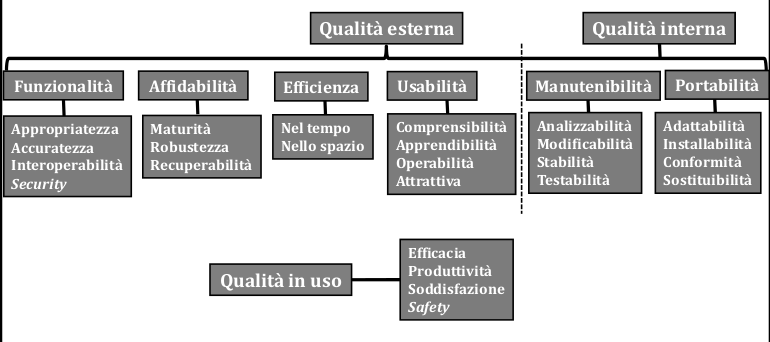
\includegraphics[width=0.78\textwidth]{img/9126}		
				\caption{Le diverse visioni delle qualità di ISO 9126:2001.}
			\end{figure} 
			
			\subsubsection{ISO 14598}	\label{14596} 
			ISO/IEC 14598:1999 fornisce il modello di valutazione che non cambia nel tempo e col contesto. La metrica che adotta è un modo per mettere in scala i numeri, per dare un significato condiviso e non ambiguo a delle caratteristiche.
			
			\subsubsection{ISO 25000}	\label{2500}
			ISO/IEC 25000:2014 è un insieme dello standard 9126 e 14598.
			Si riferisce al software, \textit{SQuaRE}: Software product Quality Requirements and Evaluation.
			
			\subsubsection{ISO 9000}	\label{9000}
			La famiglia delle norme ISO 9000 tratta i fondamenti dei modelli di qualità neutri rispetto al dominio di applicazione.
			
			\begin{figure}[H]
				\centering
				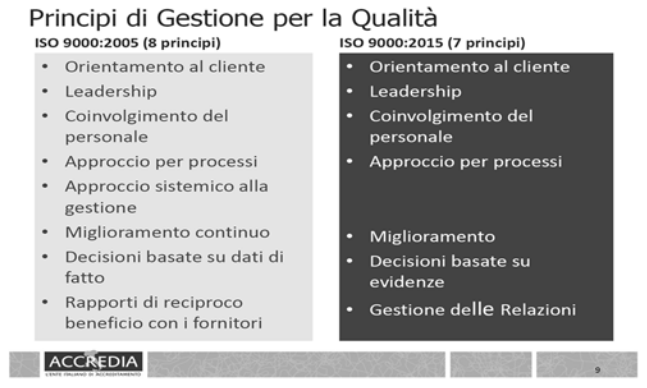
\includegraphics[width=0.78\textwidth]{img/9000}		
				\caption{I principi ISO 9000.}
			\end{figure} 
			
			\subsubsection{ISO 9001}	\label{9001}
			Applica lo standard 9000 ai sistemi produttivi. È la certificazione per la valutazione dei fornitori di prodotti o servizi. (Per il miglioramento dei risultati è stato in seguito creato il 9004).
			
			\subsubsection{ISO 15504}	\label{15504}
			\textit{Software Process Improvement Capability dEtermination} \\
			Nato per armonizzare 12207 e 9001. Metodologia di valutazione:
			\begin{itemize}
				\item Identificazione degli stakeholder: destinatari dei risultati, responsabili dei processi valutati;
				\item Scelta tra valutazione e miglioramento: risultato a uso esterno o interno, approccio formale (\textit{audit}) o meno (\textit{self-assessment}); 
				\item Definizione della portata: processi inclusi nella valutazione e indicatori di valutazione;
			\end{itemize}
					
		\subsection{STATEMENT COVERAGE}	\label{statementcoverage}	\index{Statement Coverage}
		Strumento che si ricorda quali \textit{statement} il test ha attraversato. Si ha quindi copertura al 100\% quando i test effettuati sull'unità sono sufficienti a eseguire almeno una volta tutti i comandi dell'unità con esito corretto.
					
			
		\subsection{STATO} \index{Stato} \label{stato}
		[Da Automi] è il valore assunto da variabili di stato, conseguente ad azioni precedenti su di esse (viene deciso dal Software Engineer).
		
		\subsection{STUB}	\index{Stub}	\label{stub}
		Sono dei sostituti, ovvero rappresenta ciò che è chiamato dal test ma che ancora non c'è (per esempio evita ClassNotFound).
	
		\subsection{STUDIO DI FATTIBILITÁ} \index{Studio di fattibilità} \label{studiofattibilita}
		Non é un documento pubblico ma deve rimanere agli atti come un ragionamento ben fondato. È quindi un prodotto interno e definisce il rapporto tra le parti. Si capisce qui cosa si é capaci di fare, perché innanzitutto si valutano rischi, costi e benefici nell'ottica del cliente e del fornitore. Si valuta se procedere, con l’obiettivo di restare entro un costo massimo prefissato e con le conoscenze immediatamente disponibili o un piano di formazione disponibile. Si studiano gli strumenti e le tecnologie per la realizzazione, soluzioni algoritmiche e architetturali, le piattaforme idonee all'esecuzione e il costo di produzione rispetto alla redditività. Si individuano i rischi, si valutano le scadenze temporali con conseguente studio delle risorse disponibili rispetto a quelle necessarie e si valutano delle possibili strategie alternative.
	
	
